\pagelayout{wide} % No margins
\addpart{Introduction}
\pagelayout{margin} % Restore margins

\setchapterpreamble[u]{\margintoc}
\chapter{Context and motivation}
\labch{intro:context}

\blindtext\blindtext\blindtext\blindtext\blindtext
\begin{marginfigure}[-5.5cm]
    \includegraphics[]{figures/shareholders-driven-apocalysis.png}
    \caption[Shareholders-driven apocalysis]{``Yes, the planet got destroyed. But for a beautiful moment in time, we created a lot of value for shareholders''}
    % \labfig{}
\end{marginfigure}


\blindtext\blindtext\blindtext\blindtext


\begin{figure}[htbp]
    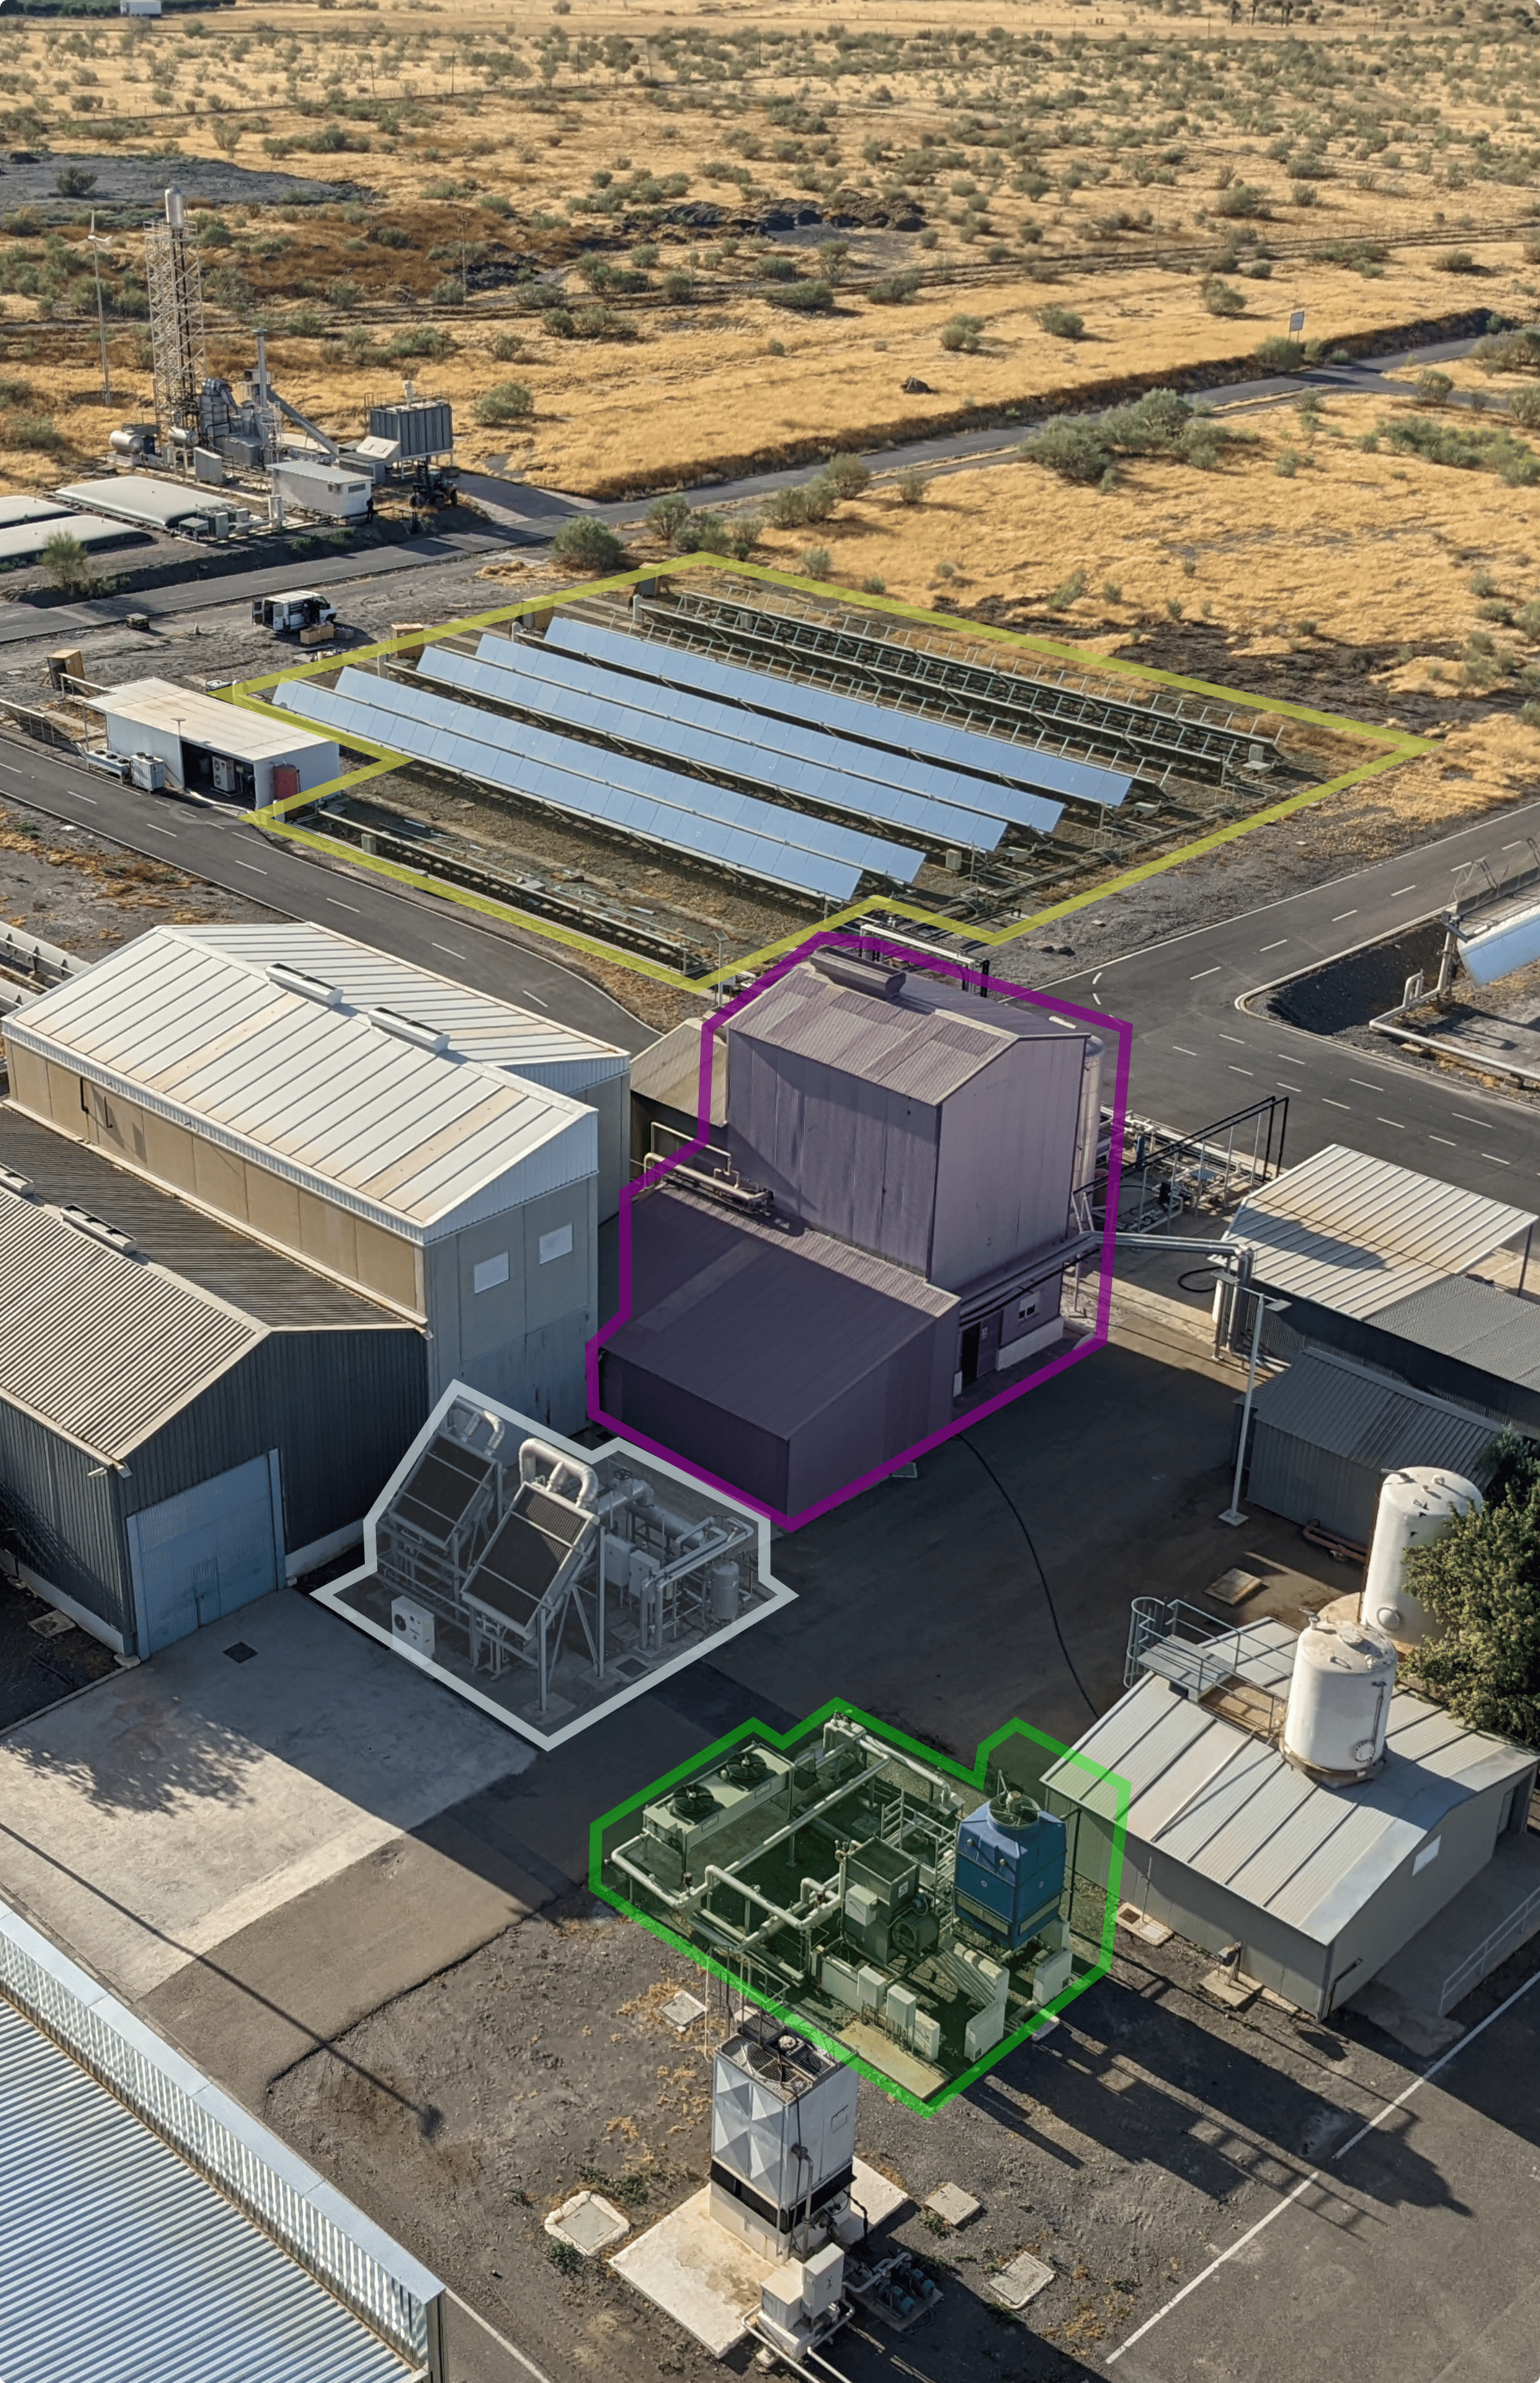
\includegraphics[width=\textwidth]{figures/pilot-plants-aerial-view.png}
    \caption[Aerial view of the pilot plants at \fullgls{psaLabel}]{Aerial view
        of the pilot plants at \fullgls{psaLabel}, Spain.\\ 
        The developments presented in this thesis have
        been developed and validated around two test-rigs: a
        \gls{ccsLabel} and a \gls{solarmedLabel} pilot plants. In the picture, the
        \gls{ccsLabel} plant is located on the left side, and the...
    }
    \labfig{intro:pilot-plants}
\end{figure}


%===================================
%===================================
%===================================
\setchapterpreamble[u]{\margintoc}
\chapter{Research plan}
\labch{intro:research-plan}


%===================================
%===================================
\section{Hypothesis}
\labsec{intro:research-plan:hypothesis}

The purpose of this thesis is to investigate the following hypotheses:

\begin{enumerate}[label=\roman*)]
    \item The cooling solution of choice in a \gls{cspLabel} plant is strongly
    dependent on the specific location of the plant, particularly on its weather
    conditions and water resources. Restricting the cooling choice to only dry
    or only wet options penalizes the overall system performance in fulfilling
    its role in the grid.

    \item Hybrid or combined cooling systems are a technically feasible
    compromise between purely wet or dry systems, but they have seen limited
    deployment due to the increased complexity in design and operation. A
    general optimization methodology for these alternative cooling solutions
    could promote their broader adoption.

    \item Thermal desalination has a role to play in alleviating water scarcity,
    not necessarily as the dominant desalination technology, but by addressing
    more niche applications. This can be achieved by making desalination more
    economically attractive through approaches such as brine mining, and/or by
    reducing water contamination through the treatment of industrial and mining
    wastewater streams.

    \item To serve such applications, thermal desalination (with emphasis on
    \gls{medLabel}) must improve in two directions: either by becoming more
    efficient through expanded operational ranges, or by adapting to
    low-temperature applications where its heat demands can partially or fully
    met using alternative sources such as low-exergy waste heat, or solar
    thermal.
\end{enumerate}

%===================================
%===================================
\section{Objectives}
\labsec{intro:research-plan:objectives}

The specific objectives and goals set out in the present research work are
divided into two main blocks, each corresponding to one of the main
contributions of the thesis\sidenote{And matches the parts in this manuscript}.
The first block (\textbf{O1}) focuses on the development of a methodology for
the modelling and optimization of combined cooling systems, while the second block
(\textbf{O2}) is centered around \gls{medLabel} systems coupled with solar
thermal plants.

\begin{enumerate}[label=\textbf{O1.\arabic*}] 
    \item Model and validate various components of combined cooling systems, as
    well as their integration into a complete combined system.  
    \item Propose a methodology for optimizing combined cooling systems.  
    \item Experimentally validate the proposed methodology.  
    \item Perform a simulation-based analysis of a representative case study
    comparing different cooling alternatives and integrating the proposed
    methodology.
\end{enumerate}
\bigskip
\begin{enumerate}[label=\textbf{O2.\arabic*}]
    \item Analyze the current performance indices and evaluation criteria used
    in thermal desalination processes.  
    \item Propose a standardized methodology for the experimental evaluation and
    determination of performance criteria in thermal desalination processes.  
    \item Design and assess basic control loops, as well as identify stable
    operating conditions to ensure the reliability of experimentally obtained
    evaluation criteria.  
    \item Experimentally evaluate improvements (\eg, nanofiltration
    pretreatment) that enhance efficiency and/or reduce costs in solar
    desalination systems.  
    \item Model and simulate multi-effect desalination plants coupled with solar
    thermal systems.  
    \item Propose a methodology to optimize the operation of solar desalination
    processes based on selected performance criteria.  
    \item Evaluate hierarchical control structures aimed at optimizing
    desalination processes coupled with solar plants.  
    \item Demonstrate that the proposed hierarchical control structures improve
    the performance indices of desalination plants coupled with solar thermal
    systems.  
\end{enumerate}

%===================================
%===================================
\section{Contributions}
\labsec{intro:research-plan:contributions}


% %===================================
% %===================================
% %===================================
% \setchapterpreamble[u]{\margintoc}
% \chapter{Contributions}
% \labch{intro:contributions}

% % Generales de la tesis, abstracto
% asdad
